\section{Измерение индуктивностей }
Измерение величины индуктивности будет проведено, если  элемент определён как резистор сопротивлением 
ниже \(2100~\Omega\).
Метод измерения основан на росте тока по формуле:

\(Il~=~Imax~\cdot~(1~-~\exp{\frac{-t}{\tau}})\) 
после включения тока. Постоянная  времени \(\tau = \frac{L}{R}\) прямо пропорциональна индуктивности~\(L\), 
и обратно пропорциональна сопротивлению~\(R\). 
Ток может измеряться косвенно по падению напряжения на измерительном сопротивлении.

К сожалению, постоянная времени будет уменьшена дополнительным, относительно высоким, 
сопротивлением \(680~\Omega\), при этом измерение небольших значений индуктивности дополнительно затрудняется 
на частоте \(8~MHz\). Чтобы получить постоянную времени, напряжение на резисторе \(680~\Omega\) будет 
контролироваться  аналоговым компаратором. Если падение напряжения на резисторе \(680~\Omega\) будет выше, 
чем напряжение внутренней опоры, то это событие будет зарегистрировано 16-битным счётчиком, который запускается 
в момент включения тока. Счётчик сохранит состояние этого события. Если счётчик переполнится, то это будет 
подсчитано программой. После наступления события превышения, счётчик будет остановлен программой, и полное 
время состояния счетчика и счётчика переполнений будет сохранено. Положительная сторона катушки будет переключена 
от VCC к GND и будет оставаться в этом состоянии, пока проверка напряжения обоих выводов не покажет отсутствие тока. 
Рисунок~\ref{fig:Inductance} показывает упрощенную схему измерения индуктивности.
\begin{figure}[H]
\centering
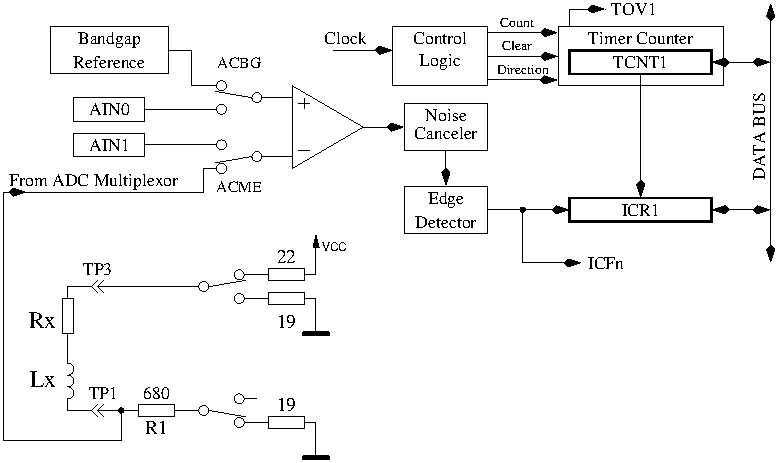
\includegraphics[width=.8\textwidth]{../FIG/Inductance.pdf}
\caption{Измерение индуктивности с компаратором}
\label{fig:Inductance}
\end{figure}

Вычисляем максимальный ток Imax, как отношение напряжения VCC к сумме всех резисторов в электрической цепи, и 
отношение опорного напряжения к максимальному напряжению на резисторе \(680~\Omega\), которое, в свою очередь, 
вычисляется по формуле \(Umax~=~Imax~\cdot~(680~+~19)\).
Индуктивность вычисляем по формуле \(L~=~-\frac{t~\cdot~Rges}{\log{(1~-~\frac{Uref}{Umax})}}\) .
Натуральный логарифм берут из таблицы. Для этого типа измерения выбрано разрешение индуктивности \(0,1~mH\).

Если величина сопротивления индуктивности будет менее \(24~\Omega\), то для того, чтобы измерить более низкие 
значения индуктивности, в цепи тока не будет использоваться резистор \(680~\Omega\). Для измерения тока будет 
использоваться только выходное сопротивление порта (\(19~\Omega\)). В этом случае пиковый ток будет больше, чем 
допустимое значение для ATmega. Поскольку это будет только в течение очень короткого промежутка времени, я не 
ожидаю повреждения портов ATmega. Для этого типа измерения выбрано разрешение индуктивности \(0,01~mH\). Чтобы 
избежать более длительного времени с чрезмерным током, дополнительное измерение с задержанным запуском счётчика 
будет всегда проводиться с резистором \(680~\Omega\). Чтобы получить более подходящие результаты измерения, 
смещение нуля 6 вычитают из счётчика, если измерение сделано без резистора \(680~\Omega\). Иначе вычитается 
смещение нуля 7 или 8.

При больших значениях индуктивности, паразитная ёмкость может вызвать быстрый рост тока, так, что компаратор 
срабатывает немедленно. Чтобы в этом случае получить значение индуктивности, измерение будет повторено с 
задержанным запуском счётчика. Этим методом аналоговым компаратором будет обнаружено напряжение, вызванное 
увеличением тока индуктивности, вместо напряжения от пика тока паразитной ёмкости. Измерения всегда делаются 
в обоих направлениях тока. Программа выберет более высокий результат измерения в том же самом направлении тока, 
а на дисплей будет выведен более низкий результат различных направлений тока.

\subsection{Результаты измерений индуктивности}
Рисунок~\ref{fig:Induct328p} показывает результаты измерения различных катушек.
Катушки выше \(1~H\) - реле или первичные обмотки силовых трансформаторов затрудняют измерения, потому что 
у железного сердечника есть остаточное намагничивание.

\begin{figure}[H]
\centering
\includegraphics[width=1.\textwidth]{../GNU/induct328pRU.pdf}
\caption{Погрешность измерения индуктивности для 15-ти различных ATmega}
\label{fig:Induct328p}
\end{figure}

\subsection{Измерение малых индуктивностей методом отбора проб}
Наименьшая индуктивность, которая может быть обнаружена при нормальном методе измерений \(0,01~mH\).
Для измерения небольшой индуктивности требуется высокая частота.
Обычный метод использует измерение скорости нарастания тока при измерении индуктивности.
Этот метод не может быть использован для метода выборки, поскольку схема измерения не использует никаких дополнительных
резисторов при испытании катушки. Ток будет расти до критически высоких значений очень быстро.
Мы можем предотвратить повреждение ATmega только с очень быстрым отключением тока.
Для выборочного метода трудно реализовать быстрое отключение и кроме того, этот критический процесс должен быть
повторен много раз в серии испытаний.

Радиолюбитель Pieter-Tjerk (PA3FWM) реализовал другой метод, чтобы получить значение индуктивности.
Параллельным подключением конденсатора к индуктивности создается резонансный контур.
С помощью короткого импульса тока эта схема возбуждается и начинает колебаться.
Используя метод дискретизации, измеряется частота этого колебания.
Так как при этом измерении один вывод катушки подключен к GND возникают две проблемы с измерением.
Отрицательное напряжение колебаний ограничивает внутренний диод защиты на порту ATmega примерно до \(0,6~V\).
По этой причине положительная часть колебаний тоже никогда не достигнет напряжения выше чем \(0,6~V\).
Кроме того АЦП в ATmega может измерять только позитивные значения напряжения.
Таким образом, все отрицательные части колебаний считываются как нулевые.
В любом случае, Pieter-Tjerk нашел решение, чтобы измерить резонансную частоту с практической точностью.
Если значение ёмкости известно и можно измерить резонансную частоту, то индуктивность может быть вычислена.
По этой причине программа калибровки нуждается в конденсаторе фиксированной ёмкости для
дальнейшего использования при измерении малых значений индуктивности.
Во время самотеста будет предложено подключить конденсатор в шаге \inquotes{\mbox{\begin{large}1 \electricC 3~10-30nF(L)\end{large}}}.
Для не откалиброванного тестера, по умолчанию, выбрано значение \(18~nF\).
Значение ёмкости параллельного конденсатора для измерения индуктивности должно быть выбрано
таким, чтобы получить резонансную частоту для всего диапазона значений измеряемых малых индуктивностей.
Конденсатор высокого качества (фольгового типа) должен быть выбран потому,
что дополнительно измеряется добротность резонансного контура путем мониторинга уменьшение амплитуды.
При использовании конденсатора высокого качества общая добротность резонансного контура будет 
определятся добротностью катушки.

Никаких дополнительных действий не требуется при параллельном подключении конденсатора.
Резонансный контур, как правило, определяется автоматически.
При обнаружении резонансного контура, отображается текст nquotas \inquotes{ if } и значение параллельной ёмкости
отображается за значением индуктивности в строке 2.
В этом случае величина сопротивления катушки отображается в конце строки 1.
Значение сопротивления катушки Вы должны проверить отдельно, измерив его без конденсатора,
потому что измерение сопротивления в резонансном контуре невозможно!
В дополнительной строке отображается измеренное значение резонансной частоты и добротность (\(Q~=\)) контура.
Если резонансный контур не обнаружен, значение сопротивления и индуктивности отображается в строке 2.
Для резонансной частоты контура определяется значение частоты и добротность катушки,
которые отображаются в дополнительной строке.

Для воздушной катушки с 6 витками и параллельно подсоединенным конденсатором \(18.1~nF\) при методе
отбора проб получен следующий результат:

\begin{verbatim}
272nH if 18.1 nF
2256kHz Q=38.7
\end{verbatim}

Такой же результат был получен с частотой от \(8~MHz\).
Аналогичный результат был также получен при измерении катушки в один виток из медной проволоки длиной \(25~cm\).
Высокое значение индуктивности, в этом примере, из-за того, что параллельно подключенный фольговый конденсатор
имеет большую собственную индуктивность.
В таблице~\ref{tab:littleInductors} показано результат измерения катушек малой индуктивности
тестером с тактовой частотой \(16~MHz\).  

\begin{table}[H]
\begin{center}
\begin{tabular}{| l | c | c | c | c | c |}
\hline
\hspace{1.5 cm} Cp= & 6.68 nF    & 11.4 nF    & 18.2 nF    & 20.3 nF    & 33.3 nF \\
Lp=           &           &           &           &           &        \\
\hline
\hline
3 витка, 13~mm & 100~nH     & 116~nH     & 108~nH     & 115~nH     & 111~nH  \\
 (91.4~nH) & 6.039~MHz  & 4.358~MHz  & 3.568~MHz  & 3.282~MHz  & 2.619~MHz \\
              & Q=29.9    & Q=15.6    & Q=49.8    & Q=12.1    & Q=31.4  \\
\hline
4 витка, 13~mm & 141~nH     & 161~nH     & 151~nH     & 152~nH     & 153~nH  \\
 (144.9~nH)     & 5.172~MHz  & 3.724~MHz  & 3.03~MHz   & 2.86~MHz   & 2.226~MHz \\
              & Q=44.8    & Q=16.0    & Q=46.2    & Q=14.6    & Q=30.5  \\
\hline
6 витков, 13~mm & 217~nH     & 232~nH     & 223~nH     & 224~nH     & 227~nH  \\
 (212.5~nH)    & 4.18~MHz   & 3.094~MHz  & 2.492~MHz  & 2.343~MHz  & 1.832~MHz \\
              & Q=30.5    & Q=18.4    & Q=43.0    & Q=15.4    & Q=31.7  \\
\hline
12 витков, 13~mm     & 547~nH     & 571~nH     & 559~nH     & 560~nH     & 566~nH  \\
 (569.5~nH)    & 2.632~MHz  & 1.973~MHz  & 1.573~MHz  & 1.491~MHz  & 1.16~MHz \\
              & Q=36.9    & Q=26.4    & Q=50.6    & Q=20.8    & Q=39.2  \\
\hline
27 витков, 11~mm & \(1.93~\mu H\) & \(1.92~\mu H\) & \(2.02~\mu H\) & \(2.00~\mu H\) & \(2.01~\mu H\)  \\
(\(1.9~\mu H\)) & 1.403~MHz  & 1.067~MHz  & 828.5~kHz  & 789.5~kHz  & 615.4~kHz \\
              & Q=36.5    & Q=33.4    & Q=43.6    & Q=26.6    & Q=34.5  \\
\hline
\(6.3~\mu H\)  & \(6.69~\mu H\) & \(6.84~\mu H\) & \(6.84~\mu H\) & \(6.82~\mu H\) & \(6.90~\mu H\)  \\
\(7.12~\mu H\) & 752.9~kHz  & 570.2~kHz  & 449.9~kHz  & 428.1~kHz  & 332.3~kHz \\
              & Q=28.5    & Q=30.5    & Q=32.3    & Q=25.5    & Q=28.3  \\
\hline
\end{tabular}
\end{center}
\caption{Результат измерения некоторых катушек с низкой индуктивностью}
\label{tab:littleInductors}
\end{table}

Для получения этих табличных значений использовались конденсаторы серии WIMA MKS, которые 
имеют низкую собственную индуктивность.
При использовании фольговых конденсаторов \(18.2~nF\), Вы получите  результат \(196~nH\)
вместо \(151~nH\) из таблицы.
Все индуктивности, кроме последней, самодельные катушки.
Значение индуктивности в скобках представляет собой вычисленные значения по размерам катушки.
Последние катушки \(6.3~\mu H\) заводские и маркированы \(6.3~\mu H\).
Но при тесте на LCR измерителе с частотой \(100~kHz\) дают результат \(7.12~\mu H\)!
Вы можете наблюдать значительные отличия добротности \(Q\) каждой катушки с разными параллельно
подключенными конденсаторами с почти одинаковым значением ёмкости.
Для катушки из 12 витков, Вы видите коэффициент добротности \(50.6\) с \(18.2~nF\)
конденсатором и коэффициент добротности \(20.8\) с \(20.3~nF\) конденсатором.
Причиной такого различия может быть программная ошибка.
Поэтому я показываю данные АЦП для катушки из 12-витков с конденсаторами \(18.2~nF\) 
и \(20.3~nF\) на рисунке~\ref{fig:W12compare} для наглядности.
Вы можете заметить четкую зависимость измерения добротности контура в приведенных данных.
Вероятно, от качества используемого конденсатора зависит точность полученного результата.


\begin{figure}[H]
\centering
\includegraphics[width=.9\textwidth]{../GNU/W12compareRU.pdf}
\caption{Данные АЦП двух резонансных контуров с той же катушкой 12 витков}
\label{fig:W12compare}
\end{figure}
